% vim: set fenc=utf-8 ft=latex encoding=utf-8
% -*- mode: latex; coding: UTF-8; -*-

\newif\ifdraft
\drafttrue

\ifdraft
	\documentclass[conference, draftclsnofoot]{IEEEtran}
	\def\baselinestretch{1}
	\setlength{\marginparwidth}{2cm}
\else
	\documentclass[conferece, final]{IEEEtran}
\fi

\usepackage[T1]{fontenc}
\usepackage[utf8]{inputenc}

\newcommand{\TheTitle}{Visualizing Release Information of Linux}
\newcommand{\TheAuthors}{Evan Wilde}
\newcommand{\TheEmails}{etcwilde@uvic.ca}
\newcommand{\TheSubject}{Digesting large amounts of commit data}
\newcommand{\TheKeywords}{Linux, git, data structures, tree data structures}

\synctex=1

\usepackage[hyphens]{url}
\urlstyle{same}

\ifdraft
	\usepackage[unicode=true,bookmarks=false,breaklinks=false,
		pdfborder={0 0 0},backref=none,colorlinks=true]{hyperref}

\else
	\usepackage[unicode=true,bookmarks=false,breaklinks=false,
		pdfborder={0 0 0},backref=none,colorlinks=false]{hyperref}
\fi

\usepackage[nospace]{cite}

% Table Support
\usepackage{dcolumn}
\usepackage{longtable}

\usepackage{balance}
\usepackage{placeins}
\usepackage{multirow}

% Extra support
\usepackage{xspace}
\usepackage{caption}

% Fix any bad-hyphenations here
\hyphenation{}

% \ifdraft
%     \usepackage[colorinlistoftodos]{todonotes}
%     \newcommand{\evan}[1]{{\color{blue}\emph{Evan Says: #1}}\xspace}
%     \newcommand{\evantodo}[1]{{\color{blue}\emph{Evan Todo: #1}}\xspace}
%     \newcommand{\dmg}[1]{{\color{blue}\emph{dmg Says: #1}}\xspace}
%     \newcommand{\dmgtodo}[1]{{\color{blue}\emph{dmg Todo: #1}}\xspace}
% \else
%     \usepackage[disable]{todonotes}
%     \newcommand{\evan}[1]{}
%     \newcommand{\evantodo}[1]{}
%     \newcommand{\dmg}[1]{}
%     \newcommand{\dmgtodo}[1]{}
% \fi
    \usepackage[colorinlistoftodos]{todonotes}

\newcommand{\tool}{{\emph Linvis}\xspace}


    \newcommand{\evan}[1]{{\color{blue}\emph{Evan Says: #1}}\xspace}
    \newcommand{\evantodo}[1]{{\color{blue}\emph{Evan Todo: #1}}\xspace}
    \newcommand{\dmg}[1]{{\color{blue}\emph{dmg Says: #1}}\xspace}
    \newcommand{\dmgtodo}[1]{{\color{blue}\emph{dmg Todo: #1}}\xspace}


%%% Local Variables:
%%% mode: plain-tex
%%% TeX-master: t
%%% End:


\begin{document}

\title{\TheTitle}
\author{
\IEEEauthorblockA{\TheAuthors}
\IEEEauthorblockN{Department of Computer Science,
                    University of Victoria, Canada.}
\IEEEauthorblockA{Email: \TheEmails}
}
\maketitle
\begin{abstract}

	With an average of over 900 top-level merges into the Linux kernel per
	release, some containing thousands of commits, many containing hundreds
	of commits, maintenance of older versions of the kernel becomes nearly
	impossible. For security, performance, and changing hardware,
	maintainers must understand the changes made to current versions of the
	kernel, and show these changes fit into older versions in order to make
	the necessary merges and modifications to the older versions. Current
	tools provide information about repositories through the directed
	acyclic graph (DAG) which is helpful for smaller projects, but with the
	scale and number of branches in the kernel, the DAG becomes
	overwhelming very quickly.

	In this paper, we present a tool that uses the dataset collected by
	German et al. to build a tool that uses a vine model instead of the
	DAG. This tool is designed to cater to the needs of users looking for a
	top-down approach, or a bottom-up approach to navigating the commit
	information of the kernel.
\end{abstract}

\begin{IEEEkeywords}
\TheKeywords
\end{IEEEkeywords}

\section{Introduction}

Maintainers of older version of the Linux kernel must sift through thousands of
commits with tools that are unable to filter and effectively visualize projects
that are of the scale of the kernel. Tools like Gitk provide users with the
full view of the DAG, showing all merges and commits. For smaller projects,
this information is useful for showing the relation between various branches.
With large modular projects, like the Linux Kernel, the DAG becomes a tangled
mess (\ref{fig:gitk}) of commits, merges, and the links between them, making it
difficult to derive an explanation of the changes.  Github provides a DAG view
for most projects, but is unable to display the DAG of projects as large as the
Linux Kernel.

\begin{figure}
	\centering
	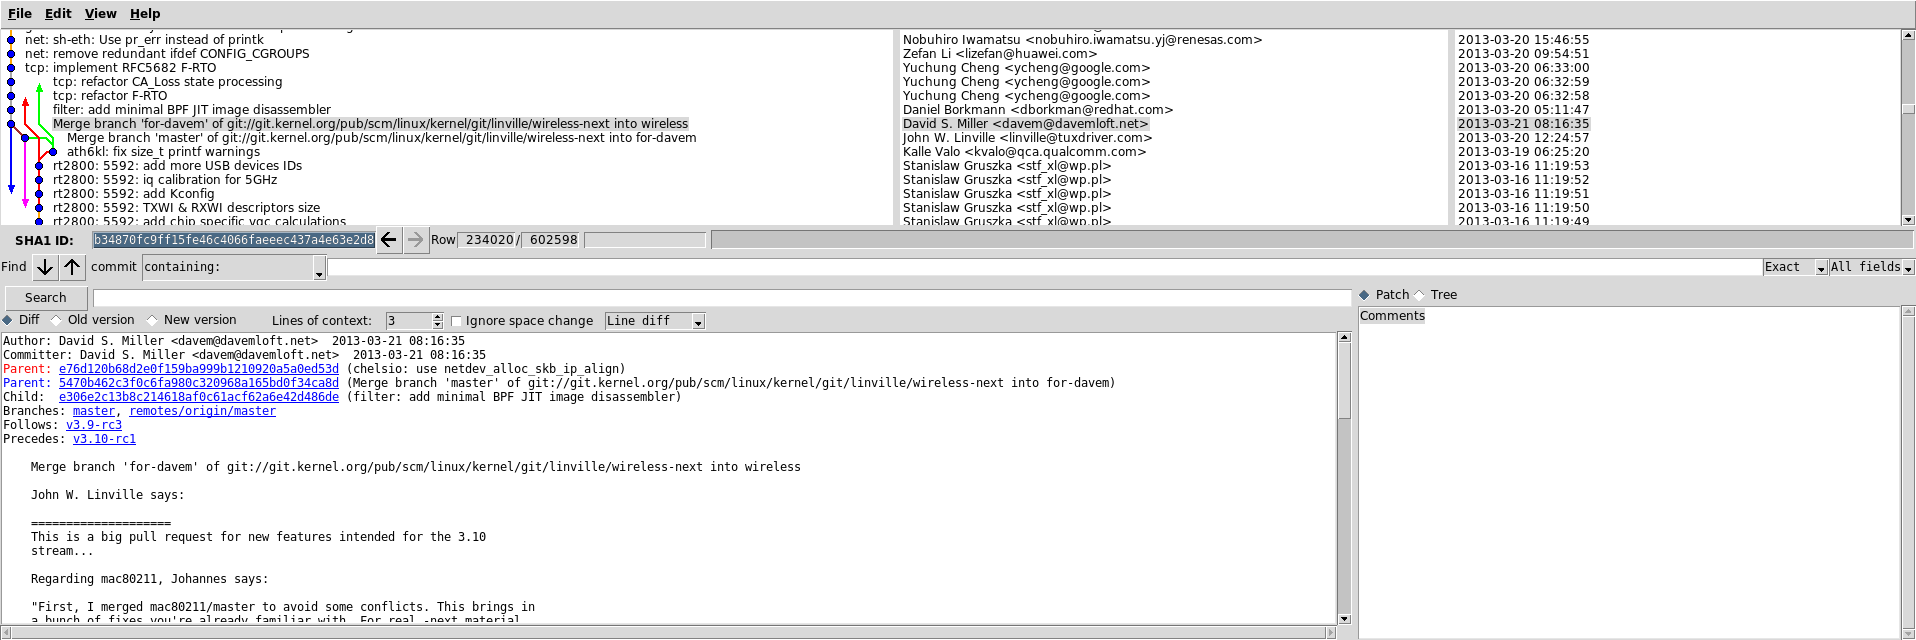
\includegraphics[width=0.47\textwidth]{figures/gitk.png}
	\caption{DAG view in Gitk}
	\label{fig:gitk}
\end{figure}

Git log, Gitk, and other similar tools only store the authored date of a
commit. A commit may be merged into the project at any time, regardless of when
the commit was authored. Because of this, performing date-range queries does
not provide meaningful results. Performing a date-range query using other tools
over the span of a release will contain results that are for previous versions
of the kernel, and may not contain all of the results for that kernel if
patches were merged after the release date.

German et al. recorded the metadata of every commit and merge in the Linux git
repository from 2012 to 2015, including data that is not stored by git. We are
able to use this information to generate sets of trees instead of a DAG. The
root of each tree is the top-level merge performed by Linus, which merges a
given commit into the kernel.

In this paper, we present the design decisions behind a web-based tool built
around a tree-based model instead of the DAG. We demonstrate the advantages of
this model over the use of the DAG. Our tool provides information about the
location of a given commit in the respective merge tree, the files edited, the
modules edited, and the commit message in a given commit or merge. The tool
allows users to apply various filters, including the release, a keyword or
phrase from the log preview, the name of the author, or the commit id. The user
can request all the top-level merges containing a commit or merge that matches
the query, or all commits and merges that match the query.

Our core model provides many advantages to other tools. Breaking the data by
merge tree removes the commits and merges of other components of the kernel
from the visualization, providing a clearer picture of what is happening in a
given merge. This model provides additional support to edited file information.

All top-level merges to a given version of the kernel are merged between the
start and release date. Our tree construction allows us to use the top-level
merges to find all merges and commits that have an effect on a given version of
the kernel. The model allows us to better provide mechanisms for performing
date-range queries, providing access to all commits that have an effect on a
given release, even if the commit comes before the start date, or the release
date.

\section{Related Work}

\subsection{Gitk}
Gitk, Gitg, and other similar git repository visualizing tools use the DAG as
the central organization. For smaller projects, this model is sufficient for
providing meaningful information, but in larger projects like the Linux kernel,
the branches become too tangled and too deep to derive any meaning from the
DAG. The DAG model allows users to go to the next commit in the chain, go to
the previous commit in the chain, or jump to the parent merge. This suggest
that Gitk and similar tools are designed for users working with a bottom-to-top
approach. With this model, it is difficult for users to see what other commits
are involved with a given merge. Gitk only provides file information on
commits, as it is unable to quickly find all files edited by a merge. It is up
to the user to remember what files were edited in each of the commits involved
in a given merge. In some of the larger merges, some containing over 1500
edited files, this task become nearly impossible.
% cid: 73287a43cc79ca06629a88d1a199cd283f42456a, 1800 commits, 1500 files
Other DAG visualization systems, like the GitHub viewer (\ref{fig:gitfail}),
are unable to provide a visualization for projects that are as large as the
kernel.

\begin{figure}[h!]
	\centering
	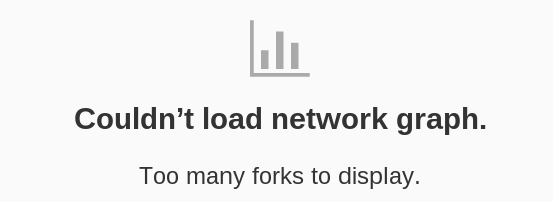
\includegraphics[width=0.45\textwidth]{figures/github_viewer.png}
	\caption{Github Failure Message}
	\label{fig:gitfail}
\end{figure}

%% Check for papers if they exist
%% This tool isn't specifically designed for showing Linux

\subsection{Treemap visualizer}
University of Maryland presented a treemap design (\ref{fig:treemap}) for
displaying all the file structure of a given version. Treemaps are good for
displaying the topology of shallow, wide trees, making it a good candidate for
displaying file systems. Treemaps are limited in what information can be
displayed. The information within the treemap does not provide clear insight on
what changes were made to the files in the given release. The treemap
visualization only provides information on where the file is located within the
filesystem. File systems and the merge tree of the kernel share many
similarities, in both cases, the representative trees are wide and shallow,
suggesting that a treemap could potentially work to visualize the commit and
merge structure of the kernel.

The treemap is unable to take into account multiple merges at the same level
with the same name. There is an additional dimension, in that the commits and
merges are ordered in time. The treemap design is unable to show the ordering
of the merges and commits.

The treemap design is also designed for working with data of differing types.
In the filesystem, there are many kinds of files.  There are text files,
scripts, images, binary files, and other types. These can be given colours
making differences stand out. There is no obvious way to assign meaningful
types to the commits such that all the commits within a given merge do not all
have the same colour.

Finally, the treemap does not provide any additional information about the
contents of each cell, only that the cell exists. The user is unable to see
their current position within the map, or if we assume that their current
position is the larges surrounding box, they can no-longer see how their
current position interacts with the rest of the system.
%% https://www.cs.umd.edu/hcil/millionvis/Treemap_Visualization_of_the_Linux_Kernel_2_5_33.html
%% Find paper for this maybe?

\begin{figure}[h!]
	\centering
	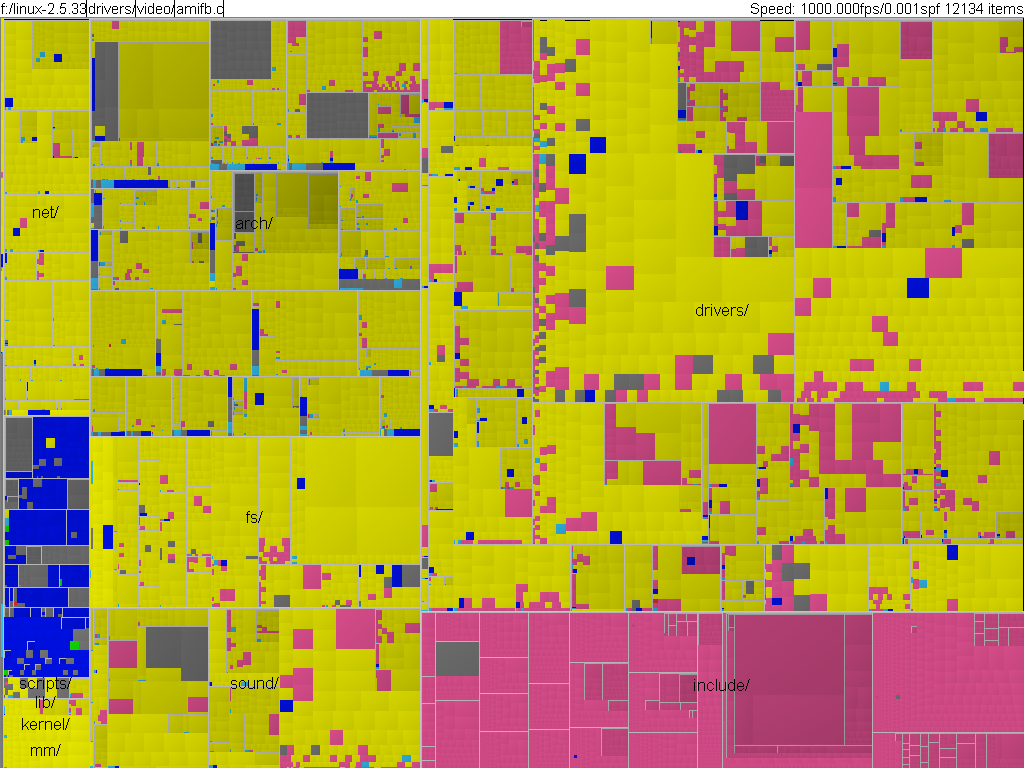
\includegraphics[width=0.47\textwidth]{figures/kernel-files.png}
	\caption{Treemap of Linux 2.5.33 file structure}
	\label{fig:treemap}
\end{figure}


\subsection{List viewer}
Moghaddam designed a web-based visualization tool displaying the chain of
merges into the kernel. There is no information on what commits are within a
given merge, or what files were edited. The visualization tool provides
information about who authored the commit and when it was authored.
\evantodo{Link to tool}
%% http://web.uvic.ca/~arasbm/gitVisualizations/linuxRGraph.html
%% Find paper for this maybe?

\begin{figure}[h!]
	\centering
	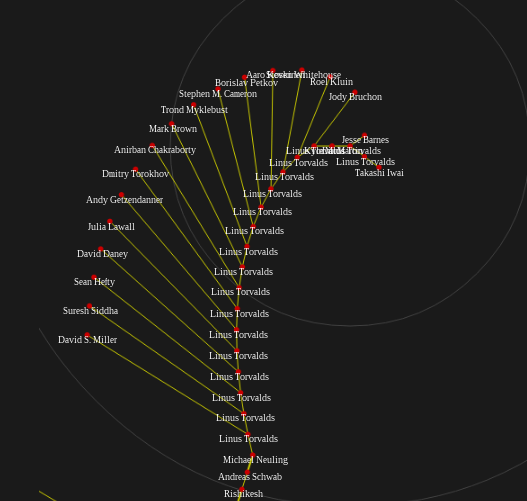
\includegraphics[width=0.47\textwidth]{figures/gitvis.png}
	\caption{List Viewer}
	\label{fig:listviewer}
\end{figure}


\section{Core Model}
Each merge may contain zero or more children of other merges or commits.
Commits have no children, and therefore are always leaf nodes, but commits
contain information about what files are edited, how many lines are edited, and
other important information.

Core Model:
	Merges are inner nodes
	Commits are leaf nodes

\section{Implementation Details}

We built a we-based tool to provide information about the kernel.
We chose to use Nginx as the main web server, postgresql as the dbms, and Flask
as the framework for generating the dynamic content.

Nginx is a high-performance, scalable HTTP and mail server. Started in 2002,
the project is much younger than the Apache project, and designed with massive
scalability and multi-processing in mind. Instead of using request-driven
threading, Nginx uses an event-driven architecture, making it more scalable,
proving itself as being the web server behind Netflix, Hulu, GitHub, Tumblr,
and many other popular sites.

Postgresql is our dbms of choice, providing fast and reliable results. There
are multiple reasons behind choosing postgresql over another dbms. The main
reason being that the dataset provided from \evantodo{paper} was generated from
a postgresql database, allowing us to import the data directly without any
further conversions. The secondary reason is that we are more familiar with
postgresql than the other systems available.

We chose the python micro-framework Flask for generating the dynamic content.
Working with flask is simple and easy.

Tool Implementation Details:
	Web Server: Nginx, Flask, postgresql
	Database: 5 tables


% \section{Design}
% 
% The goal is to build a system that allows users to easily navigate and
% understand the changes within the kernel. We provide a mechanism for performing
% searches to filter out irrelevant commits and merges, and only work with
% information that they are interested in. At the top level, the commits are
% grouped by release version. \evan{We currently do not provide a mechanism for
% checking real versions and release candidates\ldots Might be useful to at least
% note in search results section}.
% 
% 
% information as
% possible to narrow the results that we wanted to return. Right now, the largest
% set of data that a search could return is the entire set of commits that
% pertain to a given release. While this set is massive, it pales in comparison
% to every commit and merge generated for all versions of the kernel. From there,
% the design is centered around the merge tree. These are all of the commits and
% merges that eventually are merged by a top-level merge into the kernel. The
% design centers around a vine-shape. The top-level merges form a linked list,
% each node being a logical section within the kernel. These sections are defined
% by Linus. Within each of these top-level merges is a tree of merges and
% commits. The merges form the inner-nodes, and the commits form the leaf-nodes.
% 
% \evantodo{Make a vine diagram}
% % \begin{figure}[h!]
% % 	\centering
% % 	\includegraphics[width=0.47\textwidth]{figures/empty.png}
% % 	\caption{}
% % 	\label{}
% % \end{figure}
% 
% 
% Different kinds of users need to be able to use the tool differently.
% Some users may be looking for a top-down approach, trying to find the merge
% closest to the top-level merge that works with a given set of files. Other uses
% may be looking for a bottom-up approach, given a commit, what top-level merge
% includes this commit. Other users are interested in what happens in a given
% release cycle without any other requirements.
% 
% \subsection{Architecture}
% 
% % Database
% We split the data presented among five tables; commits, filesmod, logs,
% pathtomerge, and releases. The commits table stores the metadata about a given
% commit or merge. This includes the author, the authored date, the committer,
% commit date, and the file-level diff. The filesmod table stores the information
% about the files modified in a commit. We have the commit id, or cid, of the
% commit, the filename, the number of lines added and the number of lines removed
% from the file. There may be multiple files within a given commit, and there may
% be multiple commits editing the same file, the database uses an index as the
% primary key, though the primary key could be the cid, filename pair.
% 
% % Tables
% % commits
% % filesmod
% % logs
% % pathtomerge
% % releases
% 
% %
% 
% 
% \subsection{Navigation}
% 
% A user is greeted by the search screen. We break the kernel down by release,
% limiting the maximum information a user can query to help minimize being
% overwhelmed. From there, users can either search by author name, commit id, or
% keyword from the log preview. A user may also request the top-level merges that
% meet the requirements. If the checkbox is unchecked, a user is able to query
% all commits and merges that happened in the selected release cycle. If the box
% is checked, the user will get all of the top-level merges in the release cycle
% that contain a commit or merge that match the given criteria. If no criteria
% are provided and the box is checked, the user will simply be given all
% top-level merges for that release cycle. This helps separate the use-cases,
% allowing users wanting the bottom-up approach to perform searches, and users
% wanting a top-down approach to perform searches.
% 
% Once a user has found either the top-level merge or commit that they are
% interested in, they should be able to move freely between the commits and
% merges in the tree. We use three mechanisms to provide better navigation
% through the tree. The tree view, the list tree, and breadcrumbs.
% 
% The tree view provides most of the
% navigational functionality, allowing users to jump to any commit or merge in
% the current tree. The main tree view displays all the commits and merges, the
% root is the top-level merge of all the commits and merges in the group. Users
% are able to see all commits and merges of all the merges.
% 
% \evantodo{Picture of tree}
% % \begin{figure}[h!]
% % 	\centering
% % 	\includegraphics[width=0.47\textwidth]{figures/empty.png}
% % 	\caption{}
% % 	\label{}
% % \end{figure}
% 
% The list tree shows the merges and commits of the current subtree, built as
% nested lists of links to the respective commits and merges. The information in
% this tree is a subset of the main tree view, providing a method users with a
% view of what commits and merges are below the current commit or merge. If the
% current position is a commit, the tree will be empty, as commits are leaf
% nodes in the tree representation. This is designed for letting users move
% quickly down in the tree.
% 
% \evantodo{Picture of list tree}
% % \begin{figure}[h!]
% % 	\centering
% % 	\includegraphics[width=0.47\textwidth]{figures/empty.png}
% % 	\caption{}
% % 	\label{}
% % \end{figure}
% 
% 
% The breadcrumbs show the path of merges that are above the current commit or
% merge, up to the top-level merge. This allows users a fast way to move up in
% the tree.
% 
% \evantodo{Picture of breadcrumbs}
% % \begin{figure}[h!]
% % 	\centering
% % 	\includegraphics[width=0.47\textwidth]{figures/empty.png}
% % 	\caption{}
% % 	\label{}
% % \end{figure}
% 
% 
% \subsection{Information and Presentation}
% 
% Navigation is only effective if the destination contains the desired
% information. We present the commit log, what files were edited, and what
% modules were edited at a given commit or merge. Normal tools are unable to
% provide information about what files are edited in a merge because they do no
% use the tree structure. From our tree structure, we are able to traverse the
% subtree, making note of what files are edited and how many lines of code are
% added and removed at every commit.
% 
% \evantodo{Picture of files}
% % \begin{figure}[h!]
% % 	\centering
% % 	\includegraphics[width=0.47\textwidth]{figures/empty.png}
% % 	\caption{}
% % 	\label{}
% % \end{figure}
% 
% The tree views provide navigation, but are also able to present implied
% information about the depth and number of commits in a given merge.
% 
% \section{Discussion}
% 
% Our search provides mechanisms for users looking for top-down and bottom-up
% approaches. In figures \ref{fig:AndrewMortonMerges} and \ref{fig:AndrewMorton}
% we see the difference in responses when looking for the merges by Linus and the
% commits authored by Andrew Morton.
% \evantodo{Picture of results for top-down and bottom-up}
% 
% %% http://localhost:8080/search?version=Linux+3.14&commit_date_begin=&commit_date_end=&search-text=Morton&search-type=Author&merges=on
% 
% % \begin{figure}[h!]
% % 	\centering
% % 	\includegraphics[width=0.47\textwidth]{figures/empty.png}
% % 	\caption{}
% % 	\label{fig:AndrewMortonMerges}
% % \end{figure}
% %
% % \begin{figure}[h!]
% % 	\centering
% % 	\includegraphics[width=0.47\textwidth]{figures/empty.png}
% % 	\caption{}
% % 	\label{fig:AndrewMorton}
% % \end{figure}



\section{Future Work}
We have limited search functionality regarding actual files involved in
commits. If a user knows which file they are working with and what has changed
in a given file, they are unable to look specifically for commits pertaining to
that file. Adding a search filter for searching by file would allow maintainers
to perform this search.

Currently, there are still various features that have bad performance. More
work is required to get those features responding more quickly, or providing an
asynchronous mechanism and loading bars to improve user experience.

At this time, we have no evidence that our tool is able to improve the
work-flow of maintainers. We believe that the tool is able to improve the
work-flow and performance of maintainers because it is able to better assist
users because it provides cleaner mechanisms of working with the data. It is
able to provide more relevant information, while removing information that is
irrelevant to a given module or set of merges.

\end{document}
